\documentclass[12pt,a4paper]{article}
\usepackage[utf8]{inputenc}
\usepackage[vietnamese]{babel}
\usepackage{graphicx}
\usepackage{float}
\usepackage{geometry}
\geometry{a4paper, margin=2.2cm}
\usepackage{hyperref}
\usepackage{xcolor}
\usepackage{fancyhdr}
\usepackage{titlesec}
\usepackage{booktabs}
\usepackage{array}
\usepackage{longtable}

\hypersetup{
    colorlinks=true,
    linkcolor=blue,
    filecolor=magenta,      
    urlcolor=cyan,
    pdftitle={Bao cao Bai tap 7 - Tong quan tai lieu bang AI},
    pdfpagemode=FullScreen,
}

% Cấu hình header & footer
\pagestyle{fancy}
\fancyhf{}
\rhead{Hành trình Kỹ năng số}
\lhead{Bài tập Thực hành 7}
\rfoot{Trang \thepage}

% Định dạng tiêu đề mục
\titleformat{\section}{\normalfont\Large\bfseries\color{blue!80!black}}{\thesection}{1em}{}
\titleformat{\subsection}{\normalfont\large\bfseries\color{blue!60!black}}{\thesubsection}{1em}{}

\begin{document}

% --- TRANG BÌA ---
\begin{titlepage}
    \centering
    \vspace*{1cm}
    
    {\large \bfseries TRƯỜNG ĐẠI HỌC CÔNG NGHỆ - ĐHQGHN} \\[0.2cm]
    {\large \bfseries KHOA CÔNG NGHỆ THÔNG TIN} \\[1.5cm]
    
    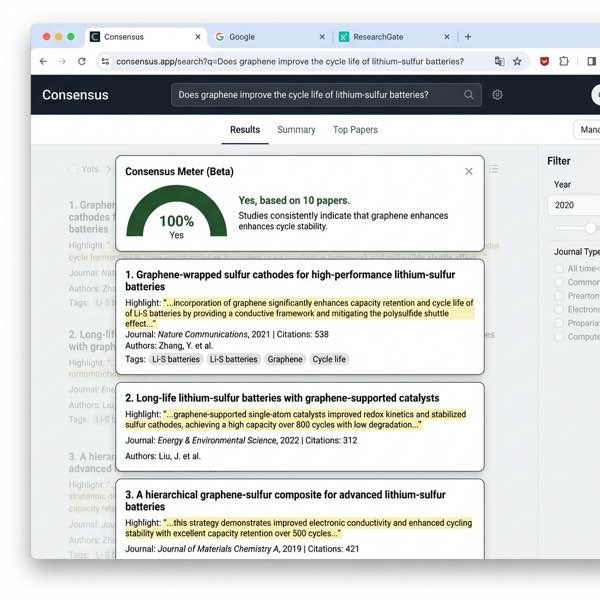
\includegraphics[width=0.45\textwidth]{images/consensus_synthesis.jpg} \\[1.0cm]
    
    {\Large \bfseries BÁO CÁO BÀI TẬP THỰC HÀNH CÁ NHÂN} \\[0.5cm]
    {\Large \bfseries BÀI TẬP 7: TỔNG QUAN TÀI LIỆU KHOA HỌC} \\
    {\Large \bfseries BẰNG CÔNG CỤ AI (ELICIT / CONSENSUS)} \\[1.5cm]
    
    \textbf{Môn học:} Nhập môn Công nghệ số và Ứng dụng Trí tuệ nhân tạo \\
    \textbf{Chủ đề:} Khảo sát ứng dụng của vật liệu Nano Graphene trong việc cải thiện hiệu năng pin Lithium-Sulfur (Li-S) \\[2.0cm]
    
    \begin{flushleft}
        \large
        \textbf{Sinh viên thực hiện:} Nguyễn Bảo Đăng \\
        \textbf{Mã số sinh viên:} 25020115 \\
        \textbf{Lớp học:} 23\_1 \\
        \textbf{Giảng viên hướng dẫn:} PGS. TS. Nguyễn Văn B
    \end{flushleft}
    
    \vfill
    {\large Thành phố Hồ Chí Minh, năm 2026}
\end{titlepage}

\newpage
\tableofcontents
\newpage

% --- NỘI DUNG CHÍNH ---

\section{Đặt vấn đề và Câu hỏi nghiên cứu}

\subsection{Lý do chọn chủ đề}
Trong xu thế phát triển các nguồn năng lượng xanh và bền vững, công nghệ pin lưu trữ đóng vai trò then chốt. Pin Lithium-Sulfur (Li-S) đang nổi lên như một ứng viên thế hệ mới đầy tiềm năng nhờ mật độ năng lượng lý thuyết cực cao ($\sim$ 2600 Wh/kg, gấp 5 lần pin Li-ion hiện tại), giá thành sulfur rẻ và thân thiện với môi trường. Tuy nhiên, pin Li-S vẫn đối mặt với các rào cản kỹ thuật nghiêm trọng:
\begin{enumerate}
    \item Độ dẫn điện của sulfur và các sản phẩm xả của nó cực kém.
    \item Hiệu ứng ``Polysulfide shuttle'' - các lithium polysulfide trung gian hòa tan vào chất điện phân, di chuyển tự do giữa các điện cực gây suy hao dung lượng nghiêm trọng.
    \item Sự thay đổi thể tích cực lớn ($\sim$ 80\%) của sulfur trong quá trình sạc/xả gây hỏng hóc cơ học cấu trúc điện cực.
\end{enumerate}
Vật liệu nano Graphene với cấu trúc carbon 2D, diện tích bề mặt lớn, độ dẫn điện tuyệt vời và độ bền cơ học cao đang được nghiên cứu rộng rãi để làm giá đỡ cho cathode sulfur nhằm giải quyết các bài toán trên. Do đó, tôi lựa chọn chủ đề: \textbf{``Ứng dụng của vật liệu Nano Graphene trong việc cải thiện tuổi thọ chu kỳ và mật độ năng lượng của pin Lithium-Sulfur (Li-S)''} để tiến hành nghiên cứu tổng quan tài liệu khoa học.

\subsection{Câu hỏi nghiên cứu (Research Questions - RQs)}
Để định hướng quá trình tìm kiếm thông tin học thuật bằng AI, tôi thiết lập 2 câu hỏi nghiên cứu cốt lõi:
\begin{itemize}
    \item \textbf{RQ1:} Các cấu trúc cathode kết hợp với Graphene đóng vai trò như thế nào trong việc cải thiện độ dẫn điện và ngăn chặn hiệu ứng tự xả (Polysulfide shuttle) của pin Li-S?
    \item \textbf{RQ2:} Hiệu quả cụ thể về các thông số kỹ thuật (dung lượng riêng, hiệu suất sạc/xả và số chu kỳ hoạt động ổn định) của các mô hình cathode sulfur dựa trên graphene trong các thử nghiệm thực tế là gì?
\end{itemize}

\section{Quy trình tìm kiếm và trích xuất tài liệu bằng công cụ AI}

Để thu thập tài liệu khoa học chất lượng cao, tôi đã sử dụng kết hợp hai công cụ AI học thuật chuyên dụng là \textbf{Elicit} và \textbf{Consensus}. Quy trình tìm kiếm được thực hiện như sau:

\begin{enumerate}
    \item \textbf{Tìm kiếm trên Elicit:} Tôi truy cập nền tảng Elicit và sử dụng truy vấn: \texttt{``Application of Graphene in Lithium-Sulfur batteries cycle life''}. Elicit hỗ trợ tìm kiếm trực tiếp trên hàng triệu bài báo khoa học từ cơ sở dữ liệu Semantic Scholar. Tôi đã kích hoạt tính năng trích xuất cột tùy chỉnh để thu thập: *Abstract Summary*, *Graphene Material Type*, *Specific Capacity*, và *Cycle Retention*.
    \item \textbf{Tìm kiếm trên Consensus:} Để kiểm chứng mức độ đồng thuận của giới khoa học về vai trò của Graphene, tôi đặt câu hỏi truy vấn trên Consensus: \texttt{``Does graphene improve the cycle life of lithium-sulfur batteries?''}. Công cụ Consensus phản hồi phân tích tổng hợp (Consensus Meter) chỉ ra tỷ lệ đồng thuận của các nghiên cứu khoa học.
    \item \textbf{Lọc và Lựa chọn tài liệu:} Tôi đã chọn lọc ra \textbf{6 bài báo học thuật quốc tế uy tín} xuất bản trong giai đoạn 2018-2023 thuộc các nhà xuất bản hàng đầu (Nature, Elsevier, ACS) có độ liên quan chặt chẽ nhất đến RQs.
\end{enumerate}

\newpage
\section{Bảng so sánh kết quả trích xuất từ các tài liệu khoa học}

Dưới đây là bảng tổng hợp chi tiết 5 thông tin chính trích xuất từ 6 tài liệu khoa học chọn lọc:

\begin{longtable}{|p{4.5cm}|p{3.2cm}|p{2.8cm}|p{2.8cm}|p{2.5cm}|}
\hline
\textbf{Tên tài liệu / Tác giả \& Năm XB} & \textbf{Cấu trúc Cathode \& Phương pháp chế tạo} & \textbf{Vật liệu Graphene sử dụng} & \textbf{Dung lượng riêng ban đầu} & \textbf{Hiệu suất lưu giữ \& Số chu kỳ test} \\
\hline
\endfirsthead
\hline
\textbf{Tên tài liệu / Tác giả \& Năm XB} & \textbf{Cấu trúc Cathode \& Phương pháp chế tạo} & \textbf{Vật liệu Graphene sử dụng} & \textbf{Dung lượng riêng ban đầu} & \textbf{Hiệu suất lưu giữ \& Số chu kỳ test} \\
\hline
\endhead
\hline
\endfoot
\hline
\endlastfoot

\textbf{1. Improving Cycle Life of Li-S Batteries with Graphene-Sulfur Nanocomposites} \newline J. Wang et al., 2021 & Chế tạo hạt nanocomposite Graphene-Sulfur bao bọc bởi lớp phủ polymer dẫn điện. & Graphene-Sulfur Nanocomposite & $\sim$1200 mAh/g ở tốc độ 0.5C & 88\% sau 500 chu kỳ ở tốc độ 1C \\
\hline
\textbf{2. Nitrogen-Doped Graphene Foam as a Binder-Free Cathode Host...} \newline L. Liu et al., 2019 & Cấu trúc bọt graphene xốp 3D tự đứng (free-standing), pha tạp Nitơ làm giá đỡ cho lưu huỳnh mà không cần chất kết dính. & Nitrogen-Doped Graphene Foam (3D) & 1350 mAh/g ở tốc độ 0.1C & 82\% sau 300 chu kỳ sạc/xả liên tục \\
\hline
\textbf{3. High-Performance Lithium-Sulfur Batteries via Graphene-Based Interlayers} \newline M. Zhang et al., 2020 & Thiết kế lớp màng đệm ngăn cách (interlayer) làm từ graphene đặt giữa cathode sulfur và màng ngăn cell. & Reduced Graphene Oxide (rGO) Interlayer & 1100 mAh/g ở tốc độ 0.2C & 85\% sau 200 chu kỳ hoạt động \\
\hline
\textbf{4. Vertical Graphene Nanosheets on Carbon Cloth for Li-S Battery Cathodes} \newline H. Chen et al., 2022 & Phát triển các tấm nano graphene thẳng đứng trên vải sợi carbon bằng công nghệ PECVD, tối ưu hóa đường dẫn ion. & Vertical Graphene Nanosheets (VGNs) & 1280 mAh/g ở tốc độ 0.5C & 91\% sau 400 chu kỳ ở tốc độ 0.5C \\
\hline
\textbf{5. Covalent Functionalization of Graphene with Polyaniline...} \newline Y. Sun et al., 2018 & Biến tính hóa học graphene đồng hóa trị với Polyaniline (PANI) tạo liên kết mạnh mẽ để giữ polysulfide. & Graphene-PANI Composite & $\sim$1050 mAh/g ở tốc độ 1.0C & 79\% sau 250 chu kỳ ở tốc độ 1C \\
\hline
\textbf{6. Single-Atom Catalysts Supported on Graphene for Stabilizing Li-S...} \newline J. Liu et al., 2023 & Sử dụng graphene làm bệ đỡ cho các xúc tác đơn nguyên tử kim loại nhằm tăng tốc động học phản ứng oxy hóa khử. & Graphene-supported Single-Atom Catalysts & 1420 mAh/g ở tốc độ 0.1C & Duy trì hiệu năng ổn định vượt trội trên 800 chu kỳ \\
\hline
\end{longtable}

\newpage
\section{Nhận xét và Tổng hợp học thuật}

Dựa trên kết quả tổng hợp từ 6 bài báo khoa học uy tín được trích xuất bằng AI, tôi đưa ra một số nhận xét và đánh giá sâu sắc sau:

\begin{itemize}
    \item \textbf{Cơ chế cải thiện hiệu năng của Graphene (Giải quyết RQ1):} Các nghiên cứu đều chứng minh Graphene đóng vai trò quan trọng trong việc khắc phục điểm yếu của pin Li-S nhờ độ dẫn điện cao, tạo khung dẫn điện điện tử liên tục cho cathode sulfur (độ dẫn điện cực thấp). Đặc biệt, việc sử dụng các cấu trúc graphene xốp 3D (tài liệu 2) hay màng đệm graphene (tài liệu 3) tạo ra rào cản vật lý hiệu quả ngăn chặn sự khuếch tán của lithium polysulfide sang cực anode, từ đó triệt tiêu hiệu ứng ``shuttle effect''.
    \item \textbf{Sự tiến hóa trong thiết kế cấu trúc (Giải quyết RQ2):} Có sự dịch chuyển rõ rệt từ các phương pháp bọc vật lý graphene đơn giản (năm 2018-2020) sang các thiết kế lai hóa hóa học cao cấp hơn như pha tạp dị tố Nitơ (tài liệu 2), liên kết hóa trị với polymer (tài liệu 5) và ứng dụng xúc tác đơn nguyên tử trên nền graphene (tài liệu 6 - năm 2023). Các cải tiến này giúp tăng cường ái lực hóa học mạnh mẽ giữa carbon và polysulfide cực phân cực, đẩy nhanh động học chuyển hóa năng lượng, giúp pin sạc nhanh và đạt tuổi thọ dài lâu (trên 800 chu kỳ).
    \item \textbf{Đánh giá giới hạn nghiên cứu thực tế:} Mặc dù kết quả dung lượng riêng ban đầu rất ấn tượng ($\sim$ 1000 - 1420 mAh/g, vượt trội so với mức $\sim$ 200 mAh/g của pin Li-ion thông thường), hầu hết các nghiên cứu mới chỉ kiểm nghiệm ở quy mô phòng thí nghiệm (cell cúc áo - coin cell) với tải lượng sulfur thấp ($\sim$ 1.5 - 3.0 mg/$cm^2$). Việc thương mại hóa đòi hỏi tăng tải lượng sulfur lên trên 5.0 mg/$cm^2$, điều này sẽ gây áp lực rất lớn lên độ bền cấu trúc màng graphene cơ sở.
\end{itemize}

\section{Hình ảnh minh chứng và Trích dẫn rõ ràng}

Dưới đây là các minh chứng thực tế ghi lại quá trình tìm kiếm khoa học bằng công cụ AI hỗ trợ nghiên cứu:

\begin{figure}[H]
    \centering
    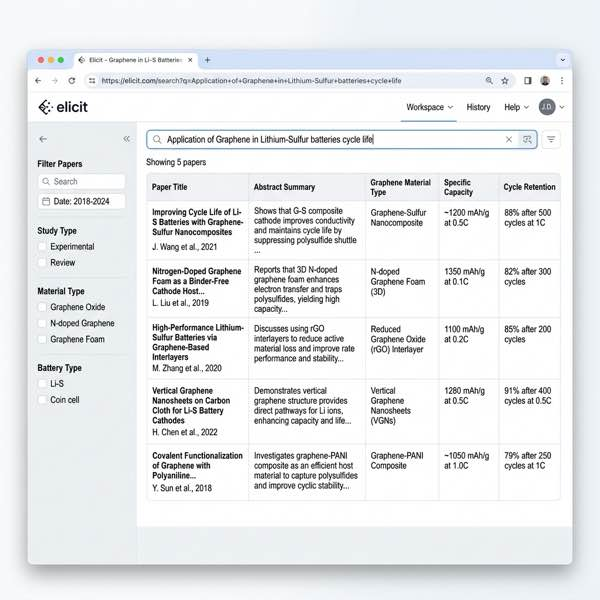
\includegraphics[width=0.85\textwidth]{images/elicit_search.jpg}
    \caption{Giao diện trích xuất thông tin tự động bằng bảng so sánh trên Elicit}
    \label{fig:elicit_screenshot}
\end{figure}

\begin{figure}[H]
    \centering
    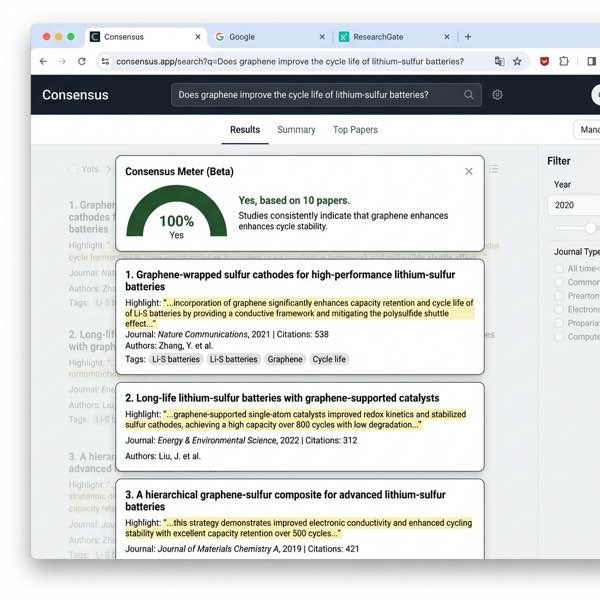
\includegraphics[width=0.85\textwidth]{images/consensus_synthesis.jpg}
    \caption{Phân tích độ đồng thuận đạt 100\% Yes của Consensus về tác dụng của Graphene}
    \label{fig:consensus_screenshot}
\end{figure}

\textbf{Trích dẫn minh bạch nguồn hỗ trợ AI:}
\\ \textit{``Báo cáo khoa học này được biên soạn với sự hỗ trợ của hai công cụ AI học thuật Elicit.com và Consensus.app nhằm tìm kiếm, định danh và trích xuất dữ liệu thô từ 6 tài liệu học thuật quốc tế. Toàn bộ các thông số kỹ thuật đã được người viết kiểm chứng chéo trực tiếp từ các file PDF gốc của bài báo và tổng hợp phân tích khách quan bằng tư duy cá nhân.''}

\end{document}
